\documentclass{article}
\usepackage{ctex}
\usepackage{graphicx}
\usepackage{amsmath}
\usepackage{indentfirst}
\usepackage{titlesec}
\usepackage{setspace}
\usepackage{subfigure}
\usepackage{caption}
\usepackage{float}
\usepackage{booktabs}
\usepackage{geometry}
\usepackage{multirow}
\usepackage{hyperref}
\hypersetup{
	colorlinks=true,
	linkcolor=blue,
	filecolor=magenta,      
	urlcolor=cyan,
	pdftitle={Overleaf Example},
	pdfpagemode=FullScreen,
}
\geometry{left=1.2cm,right=1.2cm,top=2cm,bottom=2cm}
\title{\songti \zihao{2}\bfseries HW10第16题混沌与分形}
\titleformat*{\section}{\songti\zihao{4}\bfseries}
\titleformat*{\subsection}{\songti\zihao{5}\bfseries}
\renewcommand\thesection{\arabic{section}}
\author{王启骅 PB20020580}
\begin{document}
	\maketitle
	\section{题目}
$ x_{n+1}=\lambda\sin(\pi x_n) $为迭代方程进行迭代:


(1)画出系统状态随参数 $\lambda$ 的变化图,要求在图中体现出定值状态、
倍周期分叉和混沌状态;


(2)列出各个倍周期分叉处的 $\lambda$ 值,求相应的 Feigenbaum 常数。
	\section{算法原理}
根据方程$ x_{n+1}=\lambda\sin(\pi x_n) $进行迭代,这里为了保证精度与程序运行速度,迭代5000次后认为已经达到稳定值,之后输出100个迭代结果值作为稳定解。之后将迭代结果数组输出到txt文件,用python文件pic\_chaos.py读取进行绘图。


	\section{结果}
		\begin{figure}[!h]
		
		\centering
		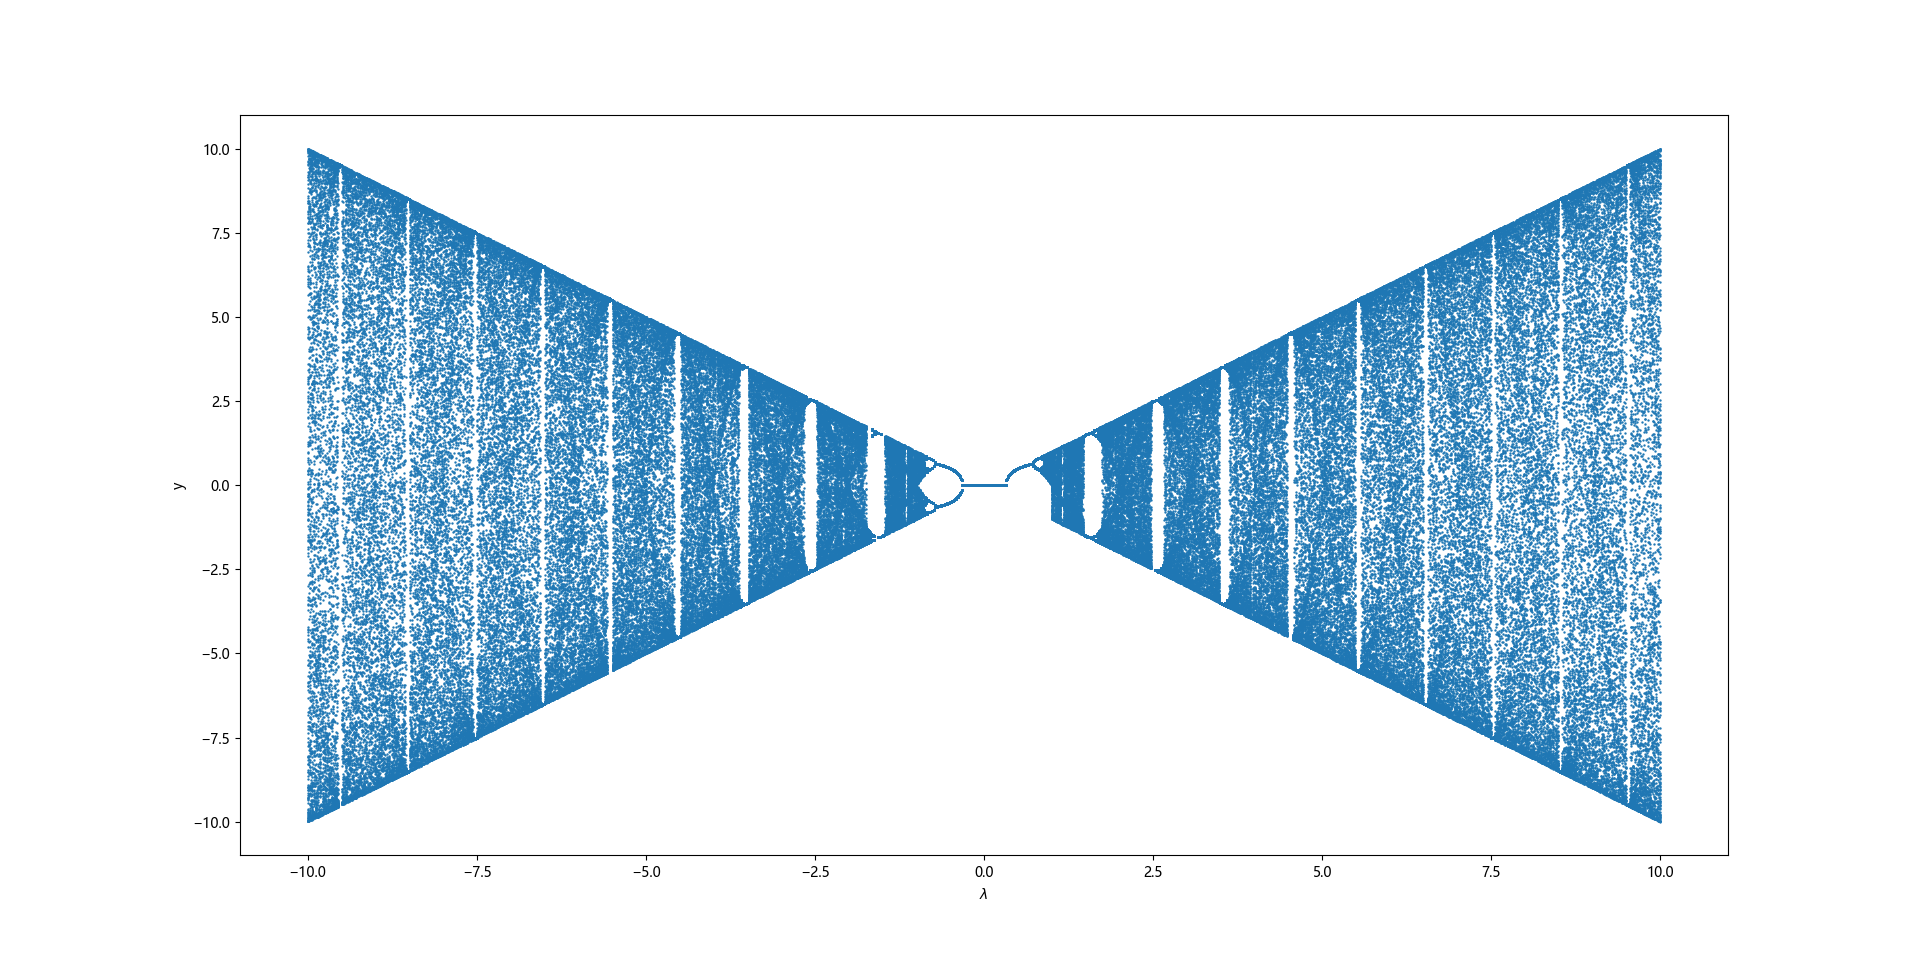
\includegraphics[scale=0.35]{result1}
		\captionsetup{font={small},labelfont=bf}
		\caption{\heiti\zihao{-5}$\lambda\in[-10,10]$迭代结果}
		\label{fig:1}
	\end{figure}
首先为了观察迭代结果的整体趋势,首先选取$ \lambda\in[-10,10] $,以$ \Delta=0.01 $作为$ \lambda $每次变化的步长。得到如图\ref{fig:1}



接下来进一步采取更小的区间,首先是$ \lambda\in[0,2] $,$ \Delta=0.0001 $下进一步细化的结果如图\ref{fig:2}
 \begin{figure}[!h]
	\centering
	\subfigure{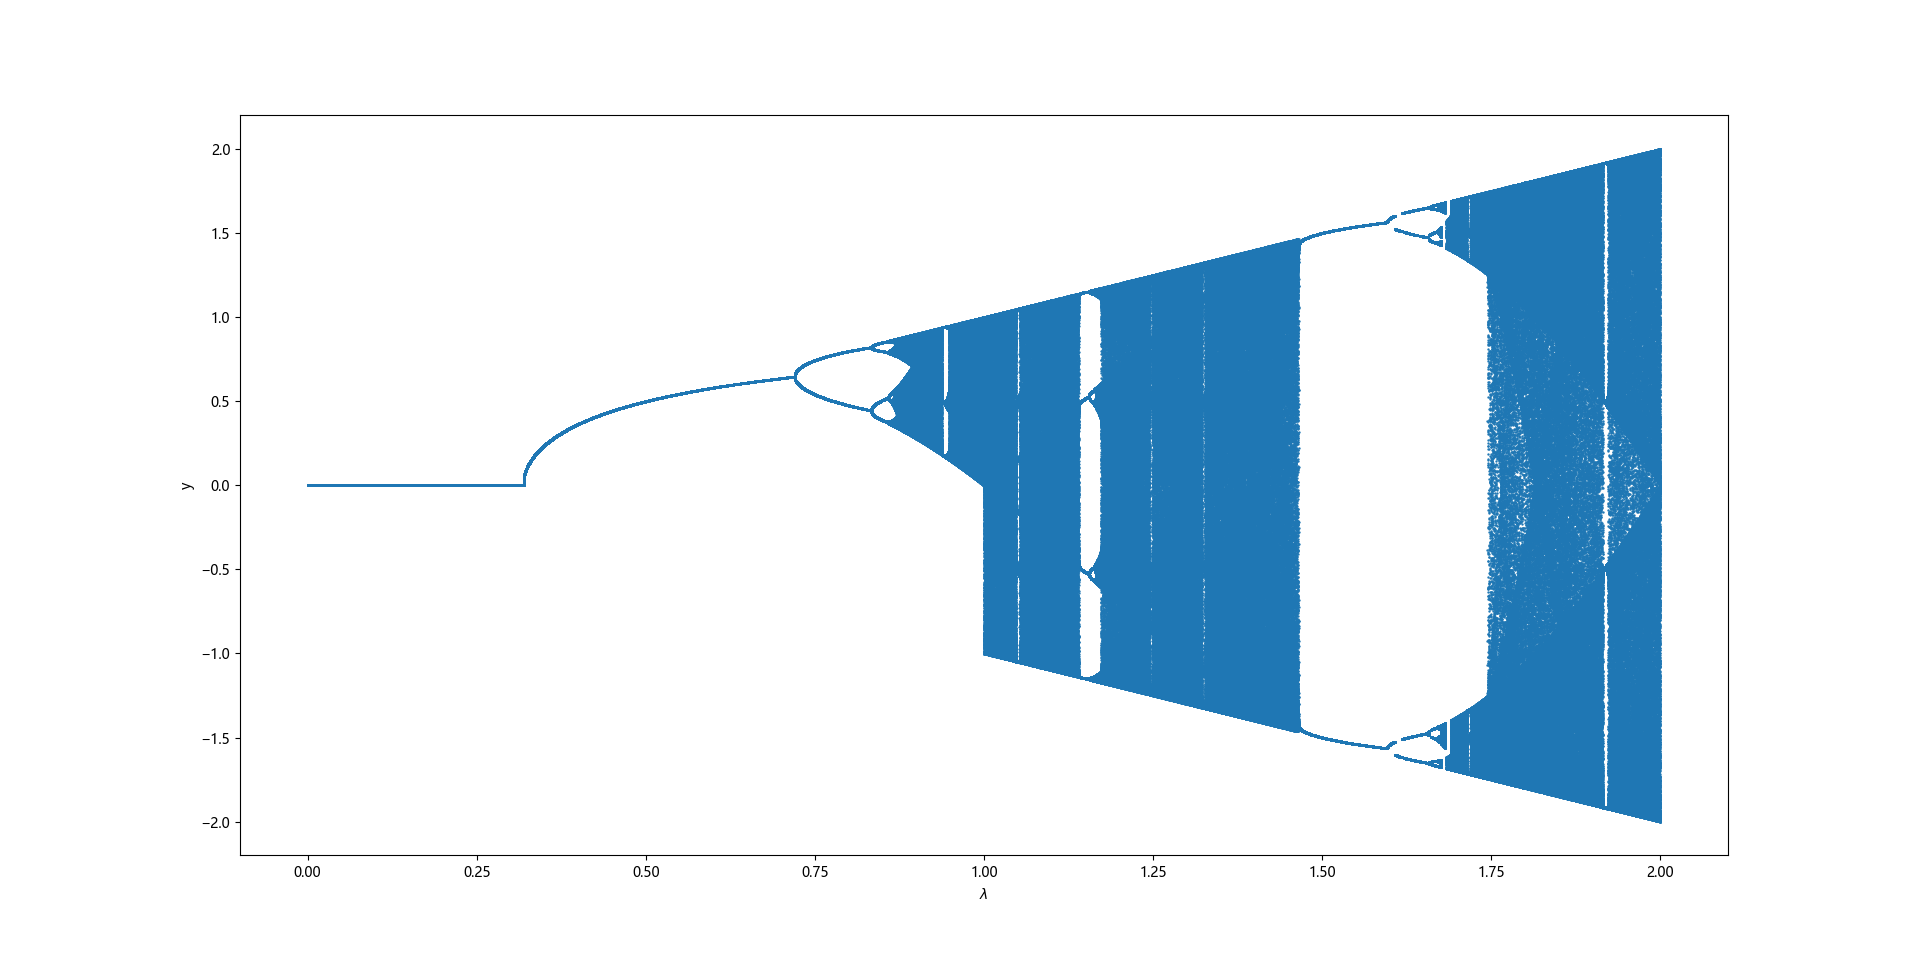
\includegraphics[scale=0.18]{result2}}
	\subfigure{	\includegraphics[scale=0.18]{result2_1}}
	
	\subfigure{\includegraphics[scale=0.18]{result2_2}}
	\subfigure{\includegraphics[scale=0.18]{result2_3}}
	\captionsetup{font={small},labelfont=bf}
	\caption{\heiti\zihao{-5}$\lambda\in[0,2]$迭代结果}
	\label{fig:2}
\end{figure}


接下来是$ \lambda\in[-2,0] $,$ \Delta=0.0001 $下进一步细化的结果如图\ref{fig:3}
\begin{figure}[!h]
	\centering
	\subfigure{\includegraphics[scale=0.18]{result3}}
	\subfigure{	\includegraphics[scale=0.18]{result3_1}}
	
	\subfigure{\includegraphics[scale=0.18]{result3_2}}
	\subfigure{\includegraphics[scale=0.18]{result3_3}}
	\captionsetup{font={small},labelfont=bf}
	\caption{\heiti\zihao{-5}$\lambda\in[-2,0]$迭代结果}
	\label{fig:3}
\end{figure}


从图中的结果可以明显的看到有在$ \lambda\in[0.6,0.9] $的范围内,有分形出现,将图片各个区域放大后可以看到明显的自相似性,当$ \lambda $进一步增大时,出现混沌,并且会偶尔出现周期窗口。同样对于$ \lambda<0 $的区域,也有分形的出现,但是由于$\lambda$时负值,导致分形具有一定的不规律性,可以由图看出存在分形数减少的曲线断开的情况。

	\subsection{Feigenbaum常数的计算}
	根据方程
	\begin{equation}
		\delta=\frac{\lambda_m-\lambda_{m-1}}{\lambda_{m+1}-\lambda_m}=4.669201
	\end{equation}
	\begin{equation}
		\alpha=\frac{d_m}{d_{m+1}}=2.502908
	\end{equation}
	
	在计算$\delta$时根据$\epsilon$作为判据,当发现$\lambda$对应的迭代结果数列中两个数的差的绝对值大于$\epsilon$时,认为两个数已经偏离,产生新的分形,从而记录新的分叉的$\lambda$值。
	
	
	然后计算$\alpha$值,这里采用x=0.5作为水平线,取该直线与每一个分形线的交点(根据盘踞$ \epsilon $判断交点位置),并取该交点与竖直方向同一$\lambda$值对应的最接近的点作为同一主枝下的分支,计算得到距离$ d_i $,然后求得每一次分形的$\alpha$ 。
	
	
	$ \delta $的计算结果输出为如下表格\ref{tab:1}
	\begin{table}[!h]
		\centering
		\captionsetup{font={small},labelfont=bf}
		\caption{\heiti\zihao{-5}$\delta$值计算结果}
		\begin{tabular}{ccc}
			\toprule
			分叉&$\lambda$&$\delta$=$\frac{\lambda_m-\lambda_{m-1}}{\lambda_{m+1}-\lambda_m}$\\
			\midrule
			1-->2& 0.7194825&\\
			2-->4& 0.8330773&4.4607507\\
			4->8 &     0.8585427     &           4.6137150\\
			 8-->16 &     0.8640622    &            4.6366767\\
			16-->32   &   0.8652526     &           4.6283048\\
			  32-->64  &    0.8655098&\\
			\bottomrule
		\end{tabular}
	\label{tab:1}
	\end{table}


计算$ \alpha $值如表\ref{tab:2}
	\begin{table}[!h]
	\centering
	\captionsetup{font={small},labelfont=bf}
	\caption{\heiti\zihao{-5}$\alpha$值计算结果}
	\begin{tabular}{ccc}
		\toprule
		分叉&$\lambda$&$\alpha$=$\frac{d_m}{d_{m+1}}$\\
		\midrule
		2&  0.2777321          &      2.5907248\\
		4&  0.1072025          &      2.5214412\\
		8 &     0.0425163      &          2.5066954\\
		16   &   0.0169611      &          2.5040370\\
		32  &     0.0067735         &       2.5041799\\
		  64   &   0.0027049&\\
		\bottomrule
	\end{tabular}
	\label{tab:2}
\end{table}


对比标准结果可见较为接近,存在的误差可能是由于$ \lambda $取值离散,且离散点下需要通过一定的有限标准$\epsilon$来判断相交情况,导致本身$\lambda$变化较小的情况下,所要求的较高的精确度,产生的误差。
\section{结论}
本次实验计算得到了分形混沌的图样,模拟验证了分形的自相似性,并寻找了分形处的$\lambda$值,计算了Feigenbaum常数与标准值进行了对比。
\end{document}